\chapter{Analysis}\label{chap:analysis}

At the beginning of this chapter, we define abstract concepts useful for discussion and formalizing the problem at hand. Following that, the requirements and use cases are stated, both of which are fundamental for proper system design. Next, possible sources of open geodata available on the Web are described, and a conceptual model for the application is proposed. Lastly, we analyze and compare competing applications tangibly related to our goals, aiming to identify the set of features essential for a reasonable user experience.

\section{Definitions}\label{sec:definitions}

To simplify further communication, we give definitions used throughout the thesis and then illustrate some of them in a real-life situation.

\begin{description}
\item[Public storage] is a read-only collection of entities accessible to all users via a predefined set of methods.
\item[Private storage] is a collection of entities accessible only to a specific user and other actors authorized by the user.
\item[Client] is an integral part of the application, allowing user interaction with both public and private storage.
\item[Keyword] is a string having an ``instance of'' relationship with a given place.
\end{description}
\begin{center}This place is an \textsf{instance of} a museum.\end{center}
\begin{description}
\item[Attribute] is a singleton or key-value pair having a ``has a'' relationship with a given place.
\end{description}
\begin{center}This museum \textsf{has a} capacity of $100$ people.\end{center}
\begin{description}
\item[Attribute filter] is a constraint imposed on a certain attribute. Only museums with a phone number and a large enough capacity would be selected by the query from the example.
\item[Place] is any location recognized by the public or private storage and associated with at least one keyword and a (possibly empty) set of attributes.
\item[Named location] is a distinguished point on the map recognized by the private storage. Possible candidates are locations with special meaning for the user, such as place of work, home, and so on.
\item[Path] is a composite structure consisting of a starting point, destination, optional waypoints in between, and a polygonal chain.
\item[Direction] is a path resulting from a search query based on an ordered sequence of locations.
\item[Category] is a composite structure consisting of a keyword and attribute filters.
\item[Categorical matching] is the process of recognizing whether a place belongs to a given category. Formally, we speak about the application of a binary function $m: V \times C \to \{ 0, 1 \}$, where $V$ is the set of places, and $C$ is the set of categories. Its value is equal to $1$ if a place has the keyword of a category and satisfies all attribute filters, and $0$ otherwise.
\item[Route] is a path resulting from a search query based on a set of categories. It~also comprises the context in which the search has been conducted.
\end{description}

Suppose a group of $N$ tourists wants to plan an excursion, starting at the~hotel, finishing in the city center, and visiting a castle and a museum. Not every facility is suitable due to the group size. Furthermore, it is advisable to make a reservation upfront by phone or other means.

The organizer marks two terminal points in a \emph{client} and configures two~\emph{cate\-gories} similar to the one below that \emph{match} only specific castles and museums.

\begin{equation*}
(
  \underbrace{\strut \textsf{museum}}_{\text{\emph{keyword}}},
  \underbrace{\strut \{ \textsf{phone}, \textsf{capacity} \geq N \}}_{\text{\emph{attribute filters}}}
)
\end{equation*}

Once the query form is prepared, a request is issued. The application operates over \emph{places} stored in the \emph{public storage} and suggests several \emph{routes}. The organizer saves one of them in their \emph{private storage} for later use.

\section{Requirements}\label{sec:requirements}

In this section, we specify the properties that our solution (hereinafter referred to as \emph{SmartWalk}) should possess by expressing functional and non-functional requirements.

Functional requirements are statements about the system that clarify the services and features it should provide to users and external systems, as well as how it should behave with respect to the surrounding environment.

On the contrary, non-functional requirements, also called quality attributes, define characteristics that improve the ability of the system to deliver functionality and meet stakeholders' expectations~\cite{glinz07}.

\subsection{Functional requirements}\label{ssec:functional-requirements}

Here, we outline the features our system implements, some implied by the goals of the thesis and others derived from the analysis of existing solutions in Section~\ref{sec:existing-solutions}.

\subsubsection*{Place search}

\begin{enumerate}[label=\textbf{F\arabic*}]\setcounter{enumi}{0}
\item\label{itm:f-search-places-common} The system allows users to search places around some center point within a crow-fly (or great circle) distance of at most \emph{15}~km.
\item\label{itm:f-search-places-center} The user can choose a center point on the map or from the stored options.
\item\label{itm:f-search-places-dist} The user is allowed to adjust a maximum distance (radius of a circle).
\item\label{itm:f-search-places-cats} The user can provide a list of categories for place matching. If the list~remains empty, the system retrieves all places within the bounding area.
\item\label{itm:f-search-places-list} The result is paginated ($5$, $10$, $20$, or $50$ places per page) and sorted by the distance in ascending order.
\item\label{itm:f-search-places-filter} The user is able to filter the result by category. Only places associated with at least one active category are listed.
\end{enumerate}

\subsubsection*{Route search}

\begin{enumerate}[label=\textbf{F\arabic*}]\setcounter{enumi}{6}
\item\label{itm:f-search-routes-automatic} The application enables users to search routes leading from a starting point to a destination with walking distance of at most \emph{30}~km.
\item\label{itm:f-search-routes-source-target} The user can choose a starting point and destination on the map or from the stored options. Furthermore, points are swappable and might be \underline{distinct}.
\item\label{itm:f-search-routes-dist} The user is allowed to adjust a maximum walking distance.
\item\label{itm:f-search-routes-cats} The user is required to provide at least one category for place matching.
\item\label{itm:f-search-routes-arrows} The user can define an order in which categories should be visited by configuring a set of \emph{arrows}. Arrows have the same meaning as the word ``before'' and \underline{are not allowed} to form cyclic dependencies. Given categories $\{ 1, 2, 3 \}$ and the only arrow $(1 \to 2)$, the following orders are valid:
\begin{equation*}3 \to 1 \to 2, \qquad 1 \to 3 \to 2, \qquad 1 \to 2 \to 3.\end{equation*}
\item\label{itm:f-search-routes-valid} The result contains only routes satisfying the following conditions:
\begin{itemize}
\item a route starts at the starting point, ends at the destination, and visits at least one place from each category,
\item the ``before'' relation is preserved for all arrows,
\item the distance of the route is less than or equal to the maximum.
\end{itemize}
\item\label{itm:f-search-routes-list} The result is paginated (one route per page) and sorted by the distance in ascending order.
\item\label{itm:f-search-routes-filter} The user can (un-)hide places associated with a selected category.
\end{enumerate}

\subsubsection*{Direction search}

\begin{enumerate}[label=\textbf{F\arabic*}]\setcounter{enumi}{14}
\item\label{itm:f-search-direcs-search} The system allows users to search directions for a given sequence of locations; a result contains those passing through all points in the given order.
\item\label{itm:f-search-direcs-append} The user can extend the sequence by selecting a point on the map, choosing from the stored options, or appending from a detailed view.
\item\label{itm:f-search-direcs-modify} The user can move points of the following entities to the sequence:
\begin{itemize}
\item routes from the result of a search query,
\item directions and routes in the private storage.
\end{itemize}
\item\label{itm:f-search-direcs-arrange} The application enables the user to rearrange points of the sequence one by one and reverse them.
\item\label{itm:f-search-direcs-list} The result is paginated (one direction per page) and sorted by the distance in ascending order.
\end{enumerate}

\subsubsection*{Entity management}

\begin{enumerate}[label=\textbf{F\arabic*}]\setcounter{enumi}{19}
\item\label{itm:f-entity-management-search} Search queries consider only entities of the public storage and ignore those stored privately.
\item\label{itm:f-entity-management-named-loc} The user can create named locations within their private storage.
\item\label{itm:f-entity-management-unique-places} For every place, the system maintains a unique persistent identifier and provides a detailed view of all information available in the public storage.
\item\label{itm:f-entity-management-jsonld} The detailed view of a place contains an embedded \acs{jsonld} representation of that place. The object should include only specific predetermined fields.
\item\label{itm:f-entity-management-partial-copy} The user can save a \emph{partial copy} of a place linked to the original object and redefine the name. Its detailed view indicates the existence of that copy.
\item\label{itm:f-entity-management-gen-traversals} The system generates routes and directions on demand without granting identifiers. Search queries for these kinds always yield ``new'' objects. The user can save them in their original state.
\item\label{itm:f-entity-management-unique-copy} If an entity of the public storage has a unique identifier, only \underline{one} copy of that object may exist in a given private storage.
\item\label{itm:f-entity-management-favorites} The application permits the user to view, edit, and delete routes, directions, copies of places, and named locations in their private storage.
\item\label{itm:f-entity-management-solid} The application enables the user to authenticate against a \acs{solid} server and activate an available pod as private storage.
\item\label{itm:f-entity-management-usable} The system supports all use cases without extra effort from the user regarding entity management and the concept of decentralization.\\[0.3em]
\emph{Rationale: To ensure the user has a gentle learning curve. Essentially, this requirement mandates the use of two interchangeable storages. Please refer to Requirement~\ref{itm:q-solid-indexeddb} for implementation details.}
\end{enumerate}

\subsubsection*{User interface}

\begin{enumerate}[label=\textbf{F\arabic*}]\setcounter{enumi}{29}
\item The system provides users the option to request their current location.
\item When configuring a category, the system suggests possible keywords based on a prefix. Once a keyword is selected, the system provides the user with the corresponding keyword-specific attribute filters and their bounds.
\item The removal of a category also resets the list of arrows.
\item The system enables users to clean up request forms and alter entered items, including points, categories, and arrows.
\item\label{itm:f-search-places-header} The result panels contain information regarding the number of objects found and summarize the input from the request form.
\end{enumerate}

\subsection{Non-functional requirements}\label{sssec:non-functional-requirements}

The quality of a software system can be evaluated in different dimensions, including performance, testability, and modifiability. Below, we list the essential attributes that our application possesses. The reasons behind these requirements and the decisions made to meet them are discussed in the following chapters.

\begin{enumerate}[label=\textbf{N\arabic*}]
\item The application follows the three-tier architectural pattern and consists of the frontend, backend, and infrastructural nodes.
\item The frontend is designed as a single-page application and written in TypeScript using the React library and Material UI components.
\item The frontend implements a panel-centric layout and provides the same level of user experience on both desktop and mobile devices.
\item\label{itm:q-solid-indexeddb} The frontend employs IndexedDB as device storage and a \acs{solid} pod as~ex\-ter\-nal storage. Both of them are instances of private storage.
\item The frontend prevents users from entering invalid input while interacting with panels and the map.
\item The map performs marker clustering if the number of drawn objects exceeds a predefined limit.
\item The backend is designed as a Web API application written in C\# using the ASP.NET Core framework and asynchronous primitives.
\item\label{itm:q-efficiency-variety} From the algorithmic point of view, the implementation of a route planner prioritizes efficiency and a variety of results over optimality.
\item The system uses MongoDB for both storing entities and facilitating search queries.
\item The application utilizes the \acs{osrm} backend as a routing engine to calculate paths and distance matrices.
\item The application maintains an in-memory data structure to index keywords and lists of corresponding attributes and their bounds.
\item The frontend communicates with the backend via \acs{api} based on the \acs{http} protocol and the \acs{json} data format.
\item\label{itm:q-response-time-places} The response time of reasonably large place search queries does not exceed \emph{1}~second on average.
\item\label{itm:q-response-time-routes} The response time of reasonably large route and direction search queries does not exceed \emph{2}~seconds on average.
\item The system integrates information from at least three data sources: OpenStreetMap datasets, Wikidata, and DBPedia.
\item The data ingestion strategy supports filtering based on bounding boxes and enables incremental updates.
\item The architecture enables horizontal scaling as the number of active users or data volume increases.
\item The solution provides a cross-platform deployment procedure optimized for running on a stand-alone personal computer.
\item The frontend is supported in Mozilla Firefox, Google Chrome, and Microsoft Edge browsers.
\item The source code depends on the existing open-source software and is published on \href{https://github.com/}{GitHub} as a monorepo, enabling easy collaboration with other developers.
\item The source code is testable, reusable, and decently documented. The solution uses standard techniques for code organization.
\end{enumerate}

\section{User stories}\label{sec:user-stories}

To justify the relevance of our application and understand the target audience, we list several examples of actors which would benefit from using it. All examples are given in the form of user stories, following the template ``\emph{As a <role>, I can <capability> so that/to <receive benefit>.}''

\begin{itemize}
\item As a self-guided tourist, I can create an itinerary providing a unique local experience to harness the full potential of my journey.
\item As an international student, I can explore my local area to fulfill everyday duties, including doctor, shop, or leisure.
\item As a family, we can visit the zoo and include a restaurant on the way home so that no one feels hungry after a long day.
\item As a tourist guide, I can create routes that pass through numerous categories to satisfy the interests and needs of different people.
\item As a person waiting for the train, I can find a short route through a souvenir shop and an ATM to ensure I return before the train departs.
\item As an information point, I can answer questions from my clients so that I always send them in the right direction.
\item As an entrepreneur, I can identify missed opportunities in a specific area to expand my business and increase my chances of success.
\item As a person looking for an apartment, I can learn more about services within walking distance to choose an option that fits my needs best.
\item As an urban planner, I can reflect on the development of areas I have been responsible for to help me improve my expertise.
\item As a culture vulture, I can look for art galleries, theaters, cinemas, and more in one request so that I do not have to explore each category separately.
\end{itemize}

\section{Roles}\label{sec:roles}

The system primarily caters to the needs of individuals and legal entities with diverse backgrounds that do not know their local area well or seek insights. It also does not support collaborative scenarios or interactions other than searching and storing results.

Therefore, we define only one role within the system, which is a \textbf{user}. Due to \ref{itm:f-entity-management-usable}, users authenticated against a \acs{solid} server behave the same way as if they were guests.

\section{Use cases}\label{sec:use-cases-analysis}

In addition to the requirements, we provide the essential use cases that users might need to perform within the system. Each consists of up to five parts: the initial state of the system, the normal flow, the final state, and optional alternatives and extensions. To grasp how use cases are organized, it may be beneficial to review Figures \ref{fig:uc-search-routes}, \ref{fig:uc-search-places}, \ref{fig:uc-search-direcs}, and \ref{fig:uc-entity-and-storage-management} before delving into implementation details. Their detailed descriptions are provided in Attachment~\ref{sec:use-cases-attached}.

% Some use cases are shared among search procedures and are considered only once.

The following use cases guarantee the ability to search for and save entities.

\begin{figure}[!h]
  \begin{minipage}{0.42\textwidth}
    \begin{itemize}
      \item \emph{\nameref{sssec:uc-select-point}}
      \item \emph{\nameref{sssec:uc-add-category}}
      \item \emph{\nameref{sssec:uc-add-arrow}}
      \item \emph{\nameref{sssec:uc-search-routes}}
    \end{itemize}
  \end{minipage}
  \hfill
  \begin{minipage}{0.56\textwidth}
    \begin{itemize}
      \item \emph{\nameref{sssec:uc-detailed-view}}
      \item \emph{\nameref{sssec:uc-save-place}}
      \item \emph{\nameref{sssec:uc-search-direcs}}
      \item \emph{\nameref{sssec:uc-modify-route}}
    \end{itemize}
  \end{minipage}
\end{figure}

Users are allowed to view, delete, and edit stored entities. The process of dele\-tion is similar to editing metadata and is therefore excluded from consideration.

\begin{figure}[!h]
  \begin{minipage}{0.42\textwidth}
    \begin{itemize}
      \item \emph{\nameref{sssec:uc-view-entity}}
    \end{itemize}
  \end{minipage}
  \hfill
  \begin{minipage}{0.56\textwidth}
    \begin{itemize}
      \item \emph{\nameref{sssec:uc-edit-entity}}
    \end{itemize}
  \end{minipage}
\end{figure}

The following use cases explain the interplay between device storage and \acs{solid} pod so that user data is never lost or compromised.

\begin{figure}[!h]
  \begin{minipage}{0.42\textwidth}
    \begin{itemize}
      \item \emph{\nameref{sssec:uc-activate-solid}}
    \end{itemize}
  \end{minipage}
  \hfill
  \begin{minipage}{0.56\textwidth}
    \begin{itemize}
      \item \emph{\nameref{sssec:uc-deactivate-solid}}
    \end{itemize}
  \end{minipage}
\end{figure}

While designing scenarios, the following principles have been applied to simplify human-computer interaction and make application behavior predictable.

\begin{itemize}
\item Actions that modify the application state, such as saving entities or adding arrows, are always bound to the corresponding dialog. The user is allowed to close the dialog as long as the action has not been confirmed. Otherwise, they should wait until the request is resolved.
\item Actions initiating a search prevent users from leaving the panel until the request is resolved.
\item Errors that appear within a dialog or panel do not corrupt its state. In other words, information entered before the error has occurred remains intact.
\end{itemize}

\clearpage

\begin{figure}
\centering
\includegraphics[width=1.00\linewidth]{img/analysis/uc-search-routes.png}
\caption{The use cases related to searching routes.}
\label{fig:uc-search-routes}
\end{figure}

\begin{figure}
\centering
\includegraphics[width=0.75\linewidth]{img/analysis/uc-search-places.png}
\caption{The use cases related to searching places.}
\label{fig:uc-search-places}
\end{figure}

\clearpage

\begin{figure}
\centering
\includegraphics[width=0.95\linewidth]{img/analysis/uc-search-direcs.png}
\caption{The use cases related to searching directions.}
\label{fig:uc-search-direcs}
\end{figure}

\begin{figure}
\centering
\includegraphics[width=0.55\linewidth]{img/analysis/uc-entity-and-storage-management.png}
\caption{The use cases related to entity and storage management.}
\label{fig:uc-entity-and-storage-management}
\end{figure}

\clearpage

\section{Data sources}\label{sec:data-sources}

We have introduced abstract concepts that form the foundation of our system and have outlined the procedures it will support. However, data is the key element that connects ideas to the real world and makes applications usable for end users. The goal of this section is to discuss the properties and internal organization of the selected sources of open geographic data. Their actual usage is tightly related to the conceptual model and is covered later in Section~\ref{sec:data-preparation}.

We will deal with two types of datasets: semi-structured and structured. The former usually has some internal organization but does not explain the meaning of individual items or constrain them. The latter is completely defined by schema or abstract model. For example, recall the code snippet with \acs{jsonld} serialization from Section~\ref{sec:linked-data}. The meaning of the property \texttt{knows} is precise in the presence of \texttt{@context} and becomes ambiguous without it.

All sources of structured data that we consider further are represented by large \emph{knowledge graphs}. Although this term is rather general~\cite{kgbook21}, our experience will be limited to publicly available \acs{http} endpoints capable of processing \acs{sparql} queries.

\subsection{OpenStreetMap}

\ac{osm}\footnote{\href{https://www.openstreetmap.org/}{https://www.openstreetmap.org/}} is a community-driven initiative to create freely available global-scale geographic data. The project was founded in $2004$ and, over the years, has become the largest dataset of its kind available on the Web, thanks to volunteers and regular contributors.

Perhaps one of the main reasons \acs{osm} has taken off so well and attracted the attention of thousands of people is that everyone can get started with minimal effort. Its conceptual data model defines the following three types of elements.

\begin{itemize}
\item \emph{Nodes} are point-like objects that either represent standalone real-world entities or are used as building blocks for other composite elements.
\item \emph{Ways} are ordered sequences of nodes suitable for modeling line features or area features, depending on whether the terminal points are distinct.
\item \emph{Relations} are the most generic elements designed to aggregate other primitives, including relations, and describe new meanings and behavior. Typical examples are polygons with holes, transportation routes, or even administrative boundaries.
\end{itemize}

Furthermore, each \acs{osm} entity could have a set of key-value pairs (\emph{tags}) attached. Both key and value are \emph{free-form text} entries. A key could occur within the same entity only once. Tag statistics are collected and published on Taginfo\footnote{\href{https://taginfo.openstreetmap.org/}{https://taginfo.openstreetmap.org/}}.

An example of a widely used pair is \texttt{tourism=museum}. One might argue that museums have a broader meaning and are not necessarily associated with tourism. That is another significant disadvantage of the \acs{osm} data model, making it hard to deal with in real applications.

To fix the problem, we could try to map tags to some \emph{ontology} or a schema. Sophox\footnote{\href{https://sophox.org/}{https://sophox.org/}} and WorldKG\footnote{\href{https://www.worldkg.org/}{https://www.worldkg.org/}} attempt to create knowledge graphs from \acs{osm} data, but none of the projects help to convert textual values to structured ones.

There are multiple options for how to obtain the \acs{osm} dataset. Full and partial dumps for selected regions are available on Geofabrik\footnote{\href{https://download.geofabrik.de/}{https://download.geofabrik.de/}} in binary and textual data formats. More customized queries are realizable via Overpass~API\footnote{\href{http://overpass-api.de/}{http://overpass-api.de/}}.

Despite incompleteness and heterogeneity, \acs{osm} remains a significant source of geographic data for our application. We were able to extract about $115000$~dis\-tinct entities, including polygons and relations, within a bounding box of Prague, the capital of the Czech Republic. Wikidata discussed just below contained about $35000$ point-like objects for the same area.

\subsection{Wikidata}\label{ssec:wikidata}

Wikidata\footnote{\href{https://www.wikidata.org/}{https://www.wikidata.org/}} is one of the largest publicly accessible sources of general-purpose structured data on the Web. The original idea behind this project was to create a database shared among other Wikimedia projects to deduplicate and interlink already existing information. The repository is maintained and extended by editors and robots. In addition, it integrates knowledge from various datasets with compatible licenses while keeping links to originals.

In Wikidata, anything --- a real-world entity or abstract concept --- can be represented by an \emph{item} with a label, description, and aliases. Each item is granted a unique, persistent identifier starting with \texttt{Q}. For example, \href{http://www.wikidata.org/entity/Q188112}{\texttt{Q188112}} denotes the National Museum in Prague.

Facts about items are expressed using property-value pairs called \emph{statements}. In the following example, the property \href{http://www.wikidata.org/prop/direct/P31}{\texttt{P31}} is translated to English as ``instance of,'' and \href{http://www.wikidata.org/entity/Q33506}{\texttt{Q33506}} stands for the concept of ``museum'' as an institution:

\begin{center}
\href{http://www.wikidata.org/entity/Q188112}{\texttt{Q188112}}${}^{\text{(item)}}$ \enspace $\rightarrow$ \enspace \href{http://www.wikidata.org/prop/direct/P31}{\texttt{P31}}${}^{\text{(property)}}$ \enspace $\rightarrow$ \enspace \href{http://www.wikidata.org/entity/Q33506}{\texttt{Q33506}}${}^{\text{(value)}}$.
\end{center}

To put it simply, a property describes a relation between an item and a value. Moreover, it restricts the data type of the value and possibly its range so that facts have a predictable structure and are easy to work with.

The data model of Wikidata is built upon \acs{rdf} but extends it with internal conventions. Please refer to Figure~\ref{fig:data-model-of-wikidata} for a detailed view of its structure as~pre\-sent\-ed in a web browser.

The purpose of a \emph{qualifier} is to provide additional context about a statement, such as the timestamp when it started being true.

More than one value may exist for a given item and property. For example, an object could be an instance of a ``museum'' and ``gallery'' simultaneously. \emph{Ranks} help to order values by relevancy.

One of the characteristics Wikidata mentions about itself in the product statement is being a secondary database. \emph{References} are intended to point to the source of information, making statements verifiable.

\begin{figure}[ht!]
\centering
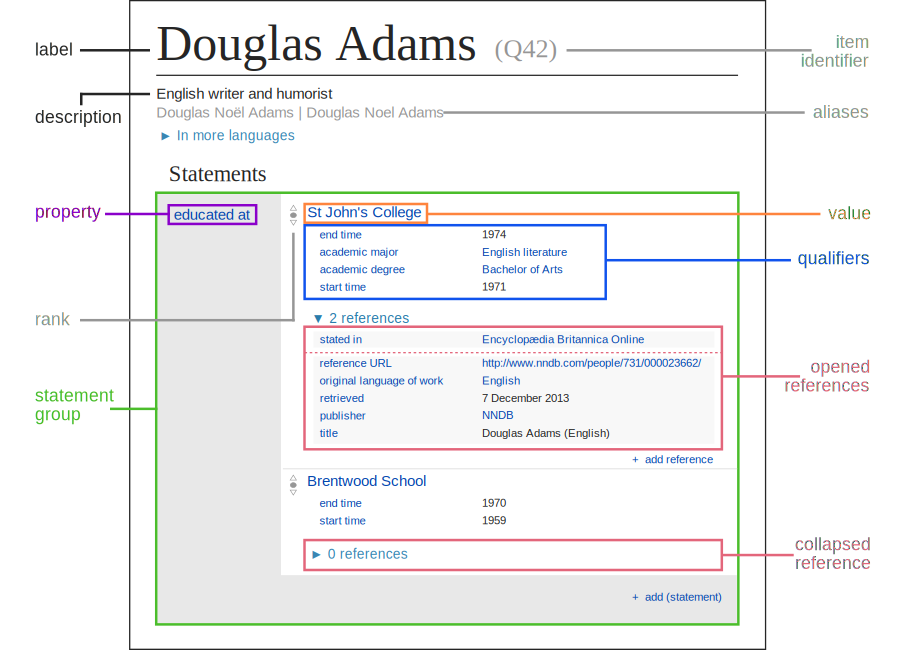
\includegraphics[width=1.0\linewidth]{img/analysis/data-model-of-wikidata.png}
\caption{Simplified data model of Wikidata~\cite{wikidata16}.}
\label{fig:data-model-of-wikidata}
\end{figure}

Wikidata follows the principles of \emph{\nameref{sec:linked-data}}; entity representation can be requested in different data formats, including \acs{jsonld}, using content negotiation. The database can also be accessed via the \acs{sparql}-based \ac{wdqs}\footnote{\href{https://query.wikidata.org/}{https://query.wikidata.org/}}. Furthermore, \acs{wdqs} offers service extensions, with the most relevant ones in the context of this thesis being geospatial \texttt{around} and \texttt{box}. The following snippet demonstrates how to retrieve all instances of museums with their locations within the bounding box of Prague.

\begin{minted}[fontsize=\footnotesize]{text}
SELECT ?wikidataId ?location WHERE {
  ?wikidataId wdt:P31/wdt:P279* wd:Q33506. # an instance of a museum
  SERVICE wikibase:box {
    ?wikidataId wdt:P625 ?location.
    bd:serviceParam wikibase:cornerSouthWest
      "Point(14.18 49.90)"^^geo:wktLiteral.
    bd:serviceParam wikibase:cornerNorthEast
      "Point(14.80 50.20)"^^geo:wktLiteral.
  }
}
\end{minted}

\subsection{DBPedia}

% http://www.dbpedia.org/resources/sparql/
% http://wikidata.dbpedia.org/develop/getting-started

DBPedia\footnote{\href{https://www.dbpedia.org/}{https://www.dbpedia.org/}} is another project in the field of \emph{\nameref{sec:linked-data}} that aims to convert Wikipedia into a structured form. Its core component, the information extraction framework initially developed by Auer et al.~\cite{auer07}, parses articles into an abstract syntax tree, performs the algorithm, and transforms the structure into an \acs{rdf} graph. This workflow implies that the resulting dataset is read-only and the only meaningful way to update it is through repeated extraction.

Although both DBPedia and Wikidata are related to Wikipedia, these projects differ in many aspects~\cite{ismayilov18}. For example, DBPedia utilizes a more general \acs{rdf} as its data model. Fortunately, if the range of the property is defined for a given triple, the extraction framework accepts only valid values.

Information from DBPedia is accessible through methods similar to Wikidata, including dumps, content negotiation, and the \acs{sparql} endpoint. Due to the generality of the extraction procedure, certain data items might be challenging~to interpret and work with. Therefore, we will use this dataset as an auxiliary source to enrich existing entities.

\section{Conceptual model}\label{sec:conceptual-model}

We have reached the point where we can interconnect abstract ideas with the available datasets. Let us show the UML class diagram of the conceptual model, depicted in Figure~\ref{fig:conceptual-model}. It mostly incorporates the entities from Section~\ref{sec:definitions} that we have already covered. Nonetheless, several aspects deserve extra attention.

All concepts evolve alongside \texttt{Keyword}, which is essential in the context of this thesis. \texttt{Place} represents the simplest form of a geographic entity that is~sen\-si\-ble to consider. Certain locations, such as tourist at\-trac\-tions, are inherently data-rich. \texttt{ExtendedPlace} helps accommodate additional information, where the \texttt{attributes} data field can be understood as a collection of key-value pairs. Moreover, we assume that each key clearly defines the data type of its value, akin to properties in Wikidata.

To search for routes, a user must provide at least one \texttt{Category}. In the initial version of the application, we implement \emph{six} types of attribute filters, formally de\-fined in Table~\ref{tab:attribute-filters}. The variable $v$ holds the result of accessing $\texttt{attributes}\left[\texttt{key}\right]$. Values for other variables are supposed to be set by the user.

\bgroup
\def\arraystretch{1.2}
\begin{table}[!h]
\centering\footnotesize
\begin{tabular}{ l l l l }
\toprule
\textbf{Filter}
  & \textbf{Variables}
    & \textbf{Predicate} \\
\midrule
Existential
  & $v : \texttt{any}$
    & defined($v$) \\
Boolean
  & $v, b : \texttt{boolean}$
    & $v = b$ \\
Numeric
  & $v, a, b : \texttt{number}$
    & $a \leq v \leq b$ \\
Textual
  & $v, t : \texttt{string}$
    & $v.\text{contains}(t)$ \\
Set (include)
  & \multirow{2}{*}{$v, s \neq \emptyset : \left\langle\texttt{string}\right\rangle$}
    & $\exists w \in s : w \in v$ \\
Set (exclude)
  & % $v, l : \left\langle\texttt{string}\right\rangle$
    & $\forall w \in s : w \not\in v$ \\
\bottomrule
\end{tabular}
\caption{Attribute filters.}
\label{tab:attribute-filters}
\end{table}
\egroup

The first type, existential, is applicable when we do not care about the shape of the value, such as an email or phone number. The meaning of the next three~rows is obvious, whereas the last two filters are less common. Suppose the user wants to have dinner in a restaurant with Czech or Slovak cuisine. Any instance of a restaurant with the attribute \texttt{cuisine} that includes \texttt{czech}, \texttt{slovak} or both would work. The last filter is the negation of the previous one.

To enable effective communication between the user and system and reduce the number of meaningless queries, bounds within an \texttt{AdviceItem} restrict ranges of their corresponding filters. The user can select only values valid for at least~one place in the public storage while configuring a category. Bounds are essential for numeric and set filters.

A careful reader might have noticed that named locations do not appear in the drawing. Instances of this type have the same structure as \texttt{Place} but are not associated with any \texttt{Keyword}. Routes and directions could still visit them.

The diagram highlights some of the elements. The green boxes are concepts of the global state and exist in the public storage. The blue entities are generated by the application in response to queries, and users can choose to store them.

\begin{figure}[!h]
\centering
\includegraphics[width=0.98\linewidth]{img/analysis/conceptual-model.png}
\caption{A UML class diagram of the conceptual model.}
\label{fig:conceptual-model}
\end{figure}

The last point we should discuss here, which eventually impacts the user interface and~the technology stack, is how to define \texttt{attributes}. Since the selected data sources offer different experiences in terms of data quality, the preprocessing phase is~nec\-es\-sary. There are at least two general approaches to this issue.

We could explicitly define keys, data types, value constraints, and mapping between our attributes and items of an external data source. This representation enables the extraction of parsable data from the \acs{osm} dataset. Moreover, resulting entities would be easier to work with for tasks like configuring categories or presenting detailed views. However, the internal structure of knowledge graphs would be underutilized.

Another method takes advantage of the fact that both knowledge graphs define the notion of a data type. For instance, property \href{http://www.wikidata.org/prop/direct/P2043}{\texttt{P2043}} in Wikidata and predicate \href{https://dbpedia.org/ontology/length}{\texttt{length}} in DBPedia both describe the ``length'' of an object. The former ex\-press\-es values in terms of \href{https://www.wikidata.org/wiki/Help:Data\_type\#quantity}{\texttt{Quantity}}, while the latter uses simple doubles.

In principle, we could ingest only property-value pairs with reasonable data types, such as boolean or double, while preparing our attributes. This approach is more generic than the previously discussed and, at the same time, problematic in several aspects.

\begin{itemize}
\item The \acs{osm} dataset remains beyond the scope; we still have to parse it.
\item A user might encounter too many attribute filters while configuring a search query.
\item A detailed view of a place would lose appeal if it had to implement a generic layout.
\item General ranges could potentially complicate the user interface. Recall the sce\-nario from \emph{\nameref{sec:definitions}}, where the group of people was looking for a museum to visit with a specific capacity requirement. In Wikidata, values~of the property \href{http://www.wikidata.org/prop/direct/P1083}{\texttt{P1083}} are constrained within the range of $0$ and $9 \times 10^5$. Con\-se\-quent\-ly, using a slider to obtain user input is no longer feasible. Instead, entered values must be validated, and errors should be reported.
\end{itemize}

Taking into account the goals of the thesis, we prioritize usability over generality. Hence, our final decision is to choose the first option and implement a fixed set of attributes.

\section{Existing solutions}\label{sec:existing-solutions}

Web maps have been around for almost three decades~\cite{plewe07}. As a result, there are implicit expectations regarding the functionality a typical application should offer and the behavior of its user interface.

In this section, we consider three types of products and compare them with our solution: commercial platforms backed by large technology companies, less popular applications implementing innovative features, and research-oriented prototypes. Table~\ref{tab:feature-comparison} summarizes the~differences and commonalities in \emph{eight} criteria.

While most websites are usable out of the box, extended capabilities might become accessible upon login. We assume that authentication has been performed.

\subsection{Mapy.cz}\label{ssec:mapy-cz}

Our starting point is Mapy.cz\footnote{\href{https://en.mapy.cz/}{https://en.mapy.cz/}}, a web mapping platform that originated in the Czech Republic. It is undoubtedly one of the most popular projects in the local market, integrating numerous industry best practices as well as several distinctive features. We use Mapy.cz as a reference point for other alternatives.

The opening page contains a vertical panel on the right side with three tabs: Search, Directions, and My~Maps; the rest is filled with raster tiles containing interactive points of interest. If the width of the viewport becomes sufficiently small, the layout switches to the mobile version. The panel moves to the bottom but keeps its layout unchanged.

The Search tab includes a search bar and category buttons. Clicking on a button has the same effect as if we had entered its label into the input. Based on provided text, autocomplete could suggest two kinds of objects that act very differently. Place items lead to the detailed view. Category items initiate search and return a list of relevant places with basic refinement filters. Filter configuration seems identical for all categories. The result is relative to the visible part of the map; shifting or zooming causes immediate recalculation. Different states of this tab are presented in Figure~\ref{fig:analysis-mapy-cz-search}.

\begin{figure}[!h]
\centering
\includegraphics[width=\linewidth]{img/analysis/mapy-cz-search.png}
\caption{Mapy.cz -- Search tab: \Circled{1} initial view, \Circled{2} autocomplete options with places and categories, \Circled{3} the results of a categorical search.}
\label{fig:analysis-mapy-cz-search}
\end{figure}

The Directions tab allows a user to construct a path in iterations. The sequence can be extended and customized in various ways; users can insert or append new points, rearrange points through drag-and-drop, and even reverse the order. The result is calculated for every sequence configuration (see Figure~\ref{fig:analysis-mapy-cz-directions} for an example). Nevertheless, this workflow suffers from all the drawbacks mentioned in the \emph{\nameref{chap:introduction}}.

\begin{figure}[!h]
\centering
\includegraphics[width=\linewidth]{img/analysis/mapy-cz-directions.png}
\caption{Mapy.cz -- Directions tab: \Circled{1} initial view, \Circled{2} a list of directions.}
\label{fig:analysis-mapy-cz-directions}
\end{figure}

Mapy.cz also supports automatic route planning, addressing one of our concerns. Given a point on the map and a maximum distance, the Circuit Route Planner\footnote{\href{https://napoveda.seznam.cz/en/circuit-route-planner-biking-and-walking/}{https://napoveda.seznam.cz/en/circuit-route-planner-biking-and-walking/}} generates a round trip and a list of tourist attractions nearby. Even though user input is reduced to two items, we can identify several drawbacks of their approach:
\begin{itemize}
\item the route is eventually circular,
\item found points might lie far from the polygonal chain,
\item the user has no control over what categories will be included in the list.
\end{itemize}

An integral part of flawless user experience is the ability to store and reuse previously obtained assets. The application enables storing all types of entities and accessing them through the My~Maps tab later. When saving a place, users can assign it any desired name. Paths in the storage are editable. Users have the option to duplicate a path by resaving it as a new entity. To enhance personalization, users can also label any position on the map and treat it as a distinct place in their collection.

\subsection{Komoot}\label{ssec:komoot}

Komoot\footnote{\href{https://www.komoot.com/}{https://www.komoot.com/}} is a web application aimed at active individuals who enjoy outdoor sports such as hiking, cycling, or running. The startup page contains two sections: Discover and Route~Planner.

The Discover section offers a community-driven tour recommendation system with filtering capabilities (duration, difficulty, elevation, etc.); routes are generated by an algorithm based on user activities\footnote{\href{https://support.komoot.com/hc/en-us/articles/360058879211}{https://support.komoot.com/hc/en-us/articles/360058879211}}.

If none of the routes meet all the requirements, users have the option to modify a discovered path or create a new one. In contrast to \emph{\nameref{ssec:mapy-cz}}, a total of \emph{22} hard\-cod\-ed category filters are available to users and activated by corresponding check\-box\-es while manually constructing a sequence of points, as shown in Figure~\ref{fig:komoot-categories}. The resulting direction can be saved and updated later. The storage functionality allows filtering by location, date, sport, or searching by name.

Outdooractive\footnote{\href{https://www.outdooractive.com/en/}{https://www.outdooractive.com/en/}} is another website with similar objectives and features.

\begin{figure}[!h]
\centering
\includegraphics[width=\linewidth]{img/analysis/komoot-categories.png}
\caption{Komoot: category filters.}
\label{fig:komoot-categories}
\end{figure}

\subsection{Kurviger}\label{ssec:kurviger}

Kurviger\footnote{\href{https://kurviger.de/about/}{https://kurviger.de/about/}} is a web application intended to cover the needs of motorcyclists. It shares several similarities with the aforementioned web pages, such as the ability to filter places by category (up to \emph{10}), store places and routes, and rename places.

Additionally, users are able to generate randomized round trips based on a starting point, compass direction, and tortuosity (refer to Figure~\ref{fig:kurviger-round-trip} for an example). Repeated searches with the same parameters yield distinct results.

Applications Naviki\footnote{\href{https://www.naviki.org/en/}{https://www.naviki.org/en/}} and cycle.travel\footnote{\href{https://cycle.travel/map}{https://cycle.travel/map}} offer a similar user experience for cyclists.

\begin{figure}[!h]
\centering
\includegraphics[width=\linewidth]{img/analysis/kurviger-round-trip.png}
\caption{Kurviger: a randomized round trip.}
\label{fig:kurviger-round-trip}
\end{figure}

% \subsection{ViaMichelin}

% ViaMichelin\footnote{\href{https://www.viamichelin.com/}{https://www.viamichelin.com/}} serves as a comprehensive travel guide equipped with an integrated map. The primary objective of this application is to provide road users with access to a wide variety of services, including restaurants, hotels, tourist attractions, and so on.

% Users can search for places based on specific categories and refine results using post-filters tailored for each category. The platform supports iterative route search, allowing users to navigate efficiently. Additionally, places associated with any of the five hardcoded categories and located very close to the path polygonal chain can be requested, as illustrated in Figure~\ref{fig:via-michelin-service-routes}.

% \begin{figure}[!h]
% \centering
% \includegraphics[width=\linewidth]{img/analysis/via-michelin-service-routes.pdf}
% \caption{ViaMichelin: activated hotels on the route}
% \label{fig:via-michelin-service-routes}
% \end{figure}

\subsection{City Trip Planner}\label{ssec:city-trip-planner}

Until now, none of the considered applications have sufficiently addressed the goals related to route search, mainly due to limited customization capabilities.

A different approach was demonstrated by Vansteenwegen et al. in~\cite{vansteenwegen11}, where they introduced an expert system, City Trip Planner, capable of planning tourist trips based on personal preferences.

In their system, users begin by entering trip constraints such as the duration of the visit, terminal points, and lunch breaks along with their interests specified through groups of keywords. Using this information, the server performs calculations and generates a multi-day trip itinerary. Additionally, places of high significance that have not been selected are presented alongside it. In subsequent iterations, users have the flexibility to improve the route by adding or removing points and request recalculations as needed.

The web page was organized as a multi-step questionnaire. The authors reported positive user feedback on the application, highlighting that the layout of the user interface posed no problems for the majority.

It is worth noting that although the City Trip Planner might no longer be available, recent projects have adopted similar principles and algorithms~\cite{herzog18, herzog19}.

\subsection{WISER}\label{ssec:wiser}

Friedman et al.~\cite{friedman12} developed and presented WISER, an experimental mobile application for iterative route search over probabilistic geospatial datasets.

We should acknowledge that some of the \emph{SmartWalk} requirements and the current algorithmic implementation of the search procedure were inspired by WISER and other articles written by its authors.

Both applications allow users to enter keywords and a set of arrows. In each iteration, WISER presents only the next place to be visited. The rationale behind this approach was that a calculated path might include waypoints the user would find irrelevant upon visiting. Instead, the system builds the route based on provided feedback. A negative response triggers a repeated calculation, while positive feedback removes the keyword from the list. The process continues as~long as at least one keyword or candidate to visit is present.

\subsection{Feature comparison}

We have discussed different solutions that are freely available on the market. Table~\ref{tab:feature-comparison} compares \emph{SmartWalk} with them based on eight criteria. In the list~be\-low, we elaborate on three less obvious ones.

\begin{description}
\item[{[Place search]}] \emph{\nameref{ssec:mapy-cz}} has the most expressive mechanism for searching places out of other alternatives. The set of keywords is unbounded, and a user can apply filters to the result (post-filtering). \emph{SmartWalk} improves its approach by allowing the user to search for multiple categories and embed filters into a query (pre-filtering).
\item[{[Route search]}] The purpose of \emph{\nameref{ssec:city-trip-planner}} was to provide tourists with a somewhat imprecise solution for navigation with no guarantees to satisfy all entered constraints. \emph{SmartWalk}, on the other hand, strives to fulfill a given task precisely. Unlike \emph{\nameref{ssec:city-trip-planner}}, \emph{SmartWalk} does not define a notion of time, as its perception is highly individual and, therefore, difficult to capture accurately.
\item[{[Saving places]}] An attached copy maintains a link to the original, whereas a~de\-tached one does the opposite.
\end{description}

\newpage

\bgroup
\def\arraystretch{1.2}
\begin{sidewaystable}[!ht]
\centering\footnotesize
\begin{threeparttable}
\begin{tabular}{ l c c c c c c }
\toprule
\textbf{Feature}
  & \textbf{\nameref{ssec:mapy-cz}}
    & \textbf{\nameref{ssec:komoot}}
      & \textbf{\nameref{ssec:kurviger}}
        & \textbf{\nameref{ssec:city-trip-planner}}
          & \textbf{\nameref{ssec:wiser}}
            & \textbf{SmartWalk} \\
\midrule
\multicolumn{7}{c}{Entity search} \\
\midrule
Place search
  & \makecell{Geocoding, unbounded \\ set of keywords, post-filters}
    & \makecell{Geocoding, bounded \\ set of keywords}
      & \makecell{Geocoding, bounded \\ set of keywords}
        & \xmark
          & \xmark
            & Categorical \\
Direction search
  & \cmark
    & \cmark
      & \cmark
        & \xmark
          & \xmark
            & \cmark \\
Route search
  & \makecell{Round, via nearby \\ attractions}
    & \makecell{Pre-calculated by \\ an algorithm}
      & \makecell{Randomized, round, \\ compass direction}
        & \makecell{Personalized, \\ time-/keyword-aware}
          & \makecell{Ordered, \\ keyword-aware}
            & \makecell{Ordered, \\ categorical} \\
\midrule
\multicolumn{7}{c}{Entity management} \\
\midrule
Data ownership
  & \makecell{Service provider}
    & \makecell{Service provider}
      & \makecell{Service provider}
        & \xmark
          & \xmark
            & \makecell{User} \\
\makecell[l]{Creating named \\ locations}
  & \cmark
    & \xmark
      & \cmark
        & \xmark
          & \xmark
            & \cmark \\
Saving places
  & \makecell{Link to an original, \\ user-defined name}
    & \makecell{Link to an original}
      & \makecell{Detached \\ partial copy}
        & \xmark
          & \xmark
            & \makecell{Attached \\ partial copy} \\
\makecell[l]{Saving routes \\ and directions}
  & \cmark
    & \cmark
      & \cmark
        & \xmark
          & \xmark
            & \cmark \\
\midrule
\multicolumn{7}{c}{User interface} \\
\midrule
Layout
  & Panel
    & Panel
      & Panel
        & Questionnaire
          & \makecell{Minimal, \\ task-oriented}
            & Panel \\
\toprule
\end{tabular}
\begin{tablenotes}
\item \cmark~denotes ``implements'', and \xmark~denotes ``does not implement.''
\end{tablenotes}
\caption{Feature comparison.}
\label{tab:feature-comparison}
\end{threeparttable}
\end{sidewaystable}
\egroup
